\fontfamily{\sfdefault}\selectfont
% XCircuit output "direct_type_1_quant.tex" for LaTeX input from direct_type_1_quant.ps
\def\putbox#1#2#3#4{\makebox[0.00000in][l]{\makebox[#1][l]{}\raisebox{\baselineskip}[0.00000in][0.00000in]{\raisebox{#2}[0.00000in][0.00000in]{\scalebox{#3}{#4}}}}}
\def\rightbox#1{\makebox[0.00000in][r]{#1}}
\def\centbox#1{\makebox[0.00000in]{#1}}
\def\topbox#1{\raisebox{-0.60\baselineskip}[0.00000in][0.00000in]{#1}}
\def\midbox#1{\raisebox{-0.20\baselineskip}[0.00000in][0.00000in]{#1}}
   \scalebox{1}{
   \normalsize
   \parbox{2.92032in}{
   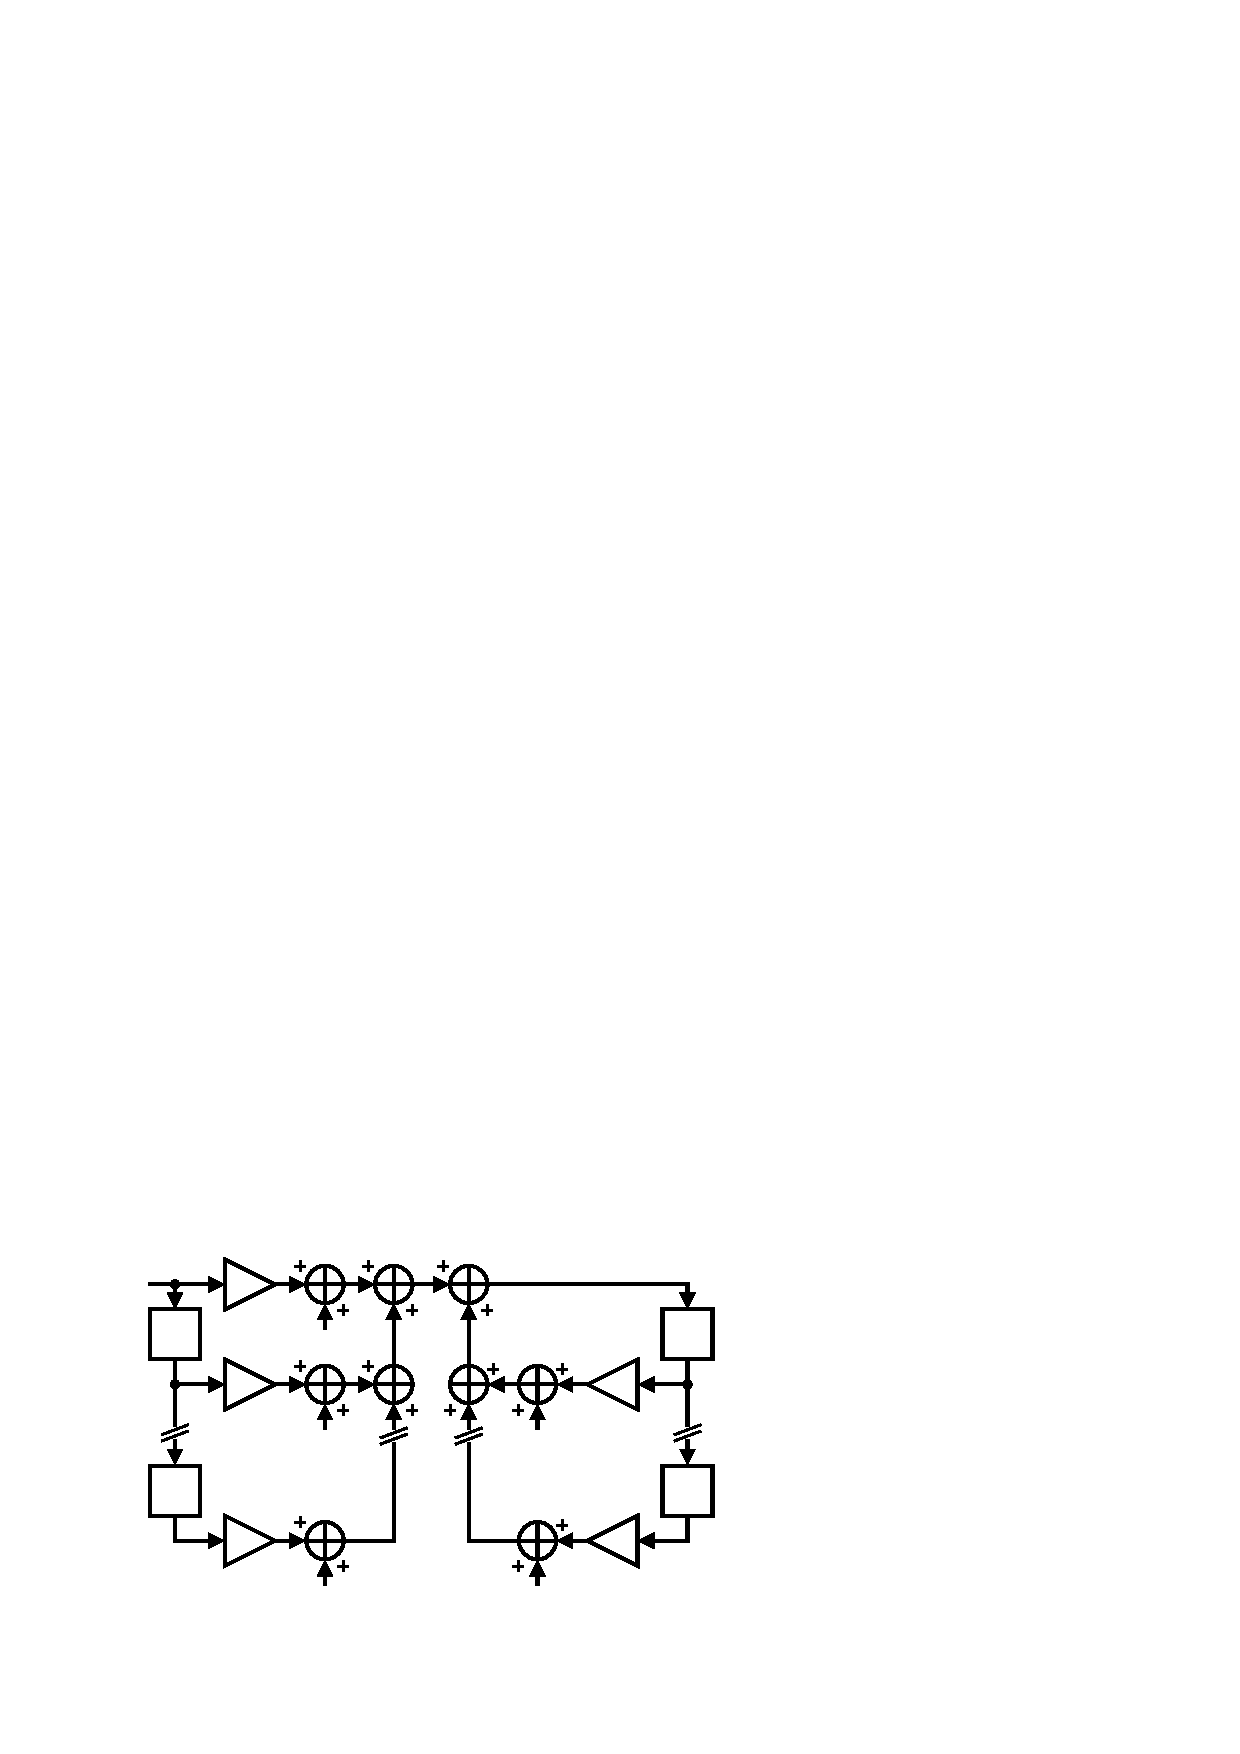
\includegraphics[scale=0.70000]{./figs/direct_type_1_quant.pdf}\\
   % translate x=936 y=1041 scale 0.38
   \putbox{0.05600in}{1.60300in}{0.96}{x[n]}%
   \putbox{2.60400in}{1.51900in}{0.96}{y[n]}%
   \putbox{0.05600in}{1.25300in}{0.96}{$z^{-1}$}%
   \putbox{0.51800in}{1.63100in}{0.96}{b$_0$}%
   \putbox{0.51800in}{1.16900in}{0.96}{b$_1$}%
   \putbox{2.44300in}{1.25300in}{0.96}{$z^{-1}$}%
   \putbox{2.44300in}{0.52500in}{0.96}{$z^{-1}$}%
   \putbox{2.03700in}{1.18300in}{0.96}{-a$_1$}%
   \putbox{2.02300in}{0.44800in}{0.96}{-a$_\mathrm{P}$}%
   \putbox{2.60400in}{1.05000in}{0.96}{y[n-1]}%
   \putbox{0.05600in}{0.52500in}{0.96}{$z^{-1}$}%
   \putbox{0.51800in}{0.43400in}{0.96}{b$_\mathrm{Z}$}%
   \putbox{0.70700in}{1.25300in}{0.96}{q$_{b_0}$[n]}%
   \putbox{0.70700in}{0.78400in}{0.96}{q$_{b_1}$[n]}%
   \putbox{0.69300in}{0.05600in}{0.96}{q$_{b_\mathrm{Z}}$[n]}%
   \putbox{1.68700in}{0.05600in}{0.96}{q$_{a_\mathrm{P}}$[n]}%
   \putbox{1.70100in}{0.78400in}{0.96}{q$_{a_1}$[n]}%
   } % close 'parbox'
   } % close 'scalebox'
   \vspace{-\baselineskip} % this is not necessary, but looks better
\fontfamily{\rmdefault}\selectfont
